%thesis.tex 
%Model LaTeX file for Ph.D. thesis at the 
%School of Mathematics, University of Edinburgh


\documentclass[11pt,a4paper,openright]{article}

%\usepackage{url,graphicx}

\usepackage{amsmath}
%\usepackage{natbib}
\usepackage{booktabs}
\usepackage{graphicx}
\usepackage{hyperref}%backref,
%\usepackage[dvips]{color}
\graphicspath{{expt/}}


\usepackage{times}
\usepackage[varg]{txfonts}

%%% Macro definitions for Commonly used symbols
\newcommand{\etas}{\ensuremath{\eta_{\mathrm{s}}}}
%\documentclass[a4paper, 11pt, draft]{Thesis} 

\usepackage{etex}
\usepackage{fixltx2e}
\usepackage{color,soul}
% This file contains macros that can be called up from connected TeX files
% It helps to summarise repeated code, e.g. figure insertion (see below).

% insert a centered figure with caption and description
% parameters 1:filename, 2:title, 3:description and label
\newcommand{\figuremacro}[3]{
	\begin{figure}[H]
		\centering
		\includegraphics[width=1\textwidth]{#1}
		\caption[#2]{\textbf{#2} - #3}
		\label{#1}
	\end{figure}
}

% insert a centered figure with caption and description AND WIDTH
% parameters 1:filename, 2:title, 3:description and label, 4: textwidth
% textwidth 1 means as text, 0.5 means half the width of the text
\newcommand{\figuremacroW}[4]{
	\begin{figure}[H]
		\centering
		\includegraphics[width=#4\textwidth]{#1}
		\caption[#2]{\textbf{#2} - #3}
		\label{#1}
	\end{figure}
}

% insert a figure with sub figures caption and description
% parameters 1:filename_1, 3:title and descriptionl_1,
% 3:filename_2, 4:title and descriptionl_2,  
% 5:title_main, 6:description and label_main,
% Each subfigure has its own caption
\newcommand{\figuremacroSubTwo}[6]{
	\begin{figure}[H]
	        \centering
		\begin{minipage}[b]{0.475\textwidth}
			\centering
			\includegraphics[width=\textwidth]{#1}
			\subcaption{#2}
		\end{minipage}%
		~
		\begin{minipage}[b]{0.475\textwidth}
			\centering
			\includegraphics[width=\textwidth]{#3}
			\subcaption{#4}
		\end{minipage}%
		\caption[#5]{\textbf{#5} - #6}
		\label{#5}
	\end{figure}
}

% insert a figure with sub figures caption and description
% parameters 1:filename_1, 3:title and descriptionl_1,
% 3:filename_2, 4:title and descriptionl_2,  
% 5:title_main, 6:description and label_main,
% Each subfigure has its own caption
\newcommand{\figuremacroSubTwoBS}[6]{
	\begin{figure}[H]
	        \centering
		\begin{minipage}[b]{0.3\textwidth}
			\centering
			\includegraphics[width=\textwidth]{#1}
			\subcaption{#2}
		\end{minipage}%
		~
		\begin{minipage}[b]{0.65\textwidth}
			\centering
			\includegraphics[width=\textwidth]{#3}
			\subcaption{#4}
		\end{minipage}%
		\caption[#5]{\textbf{#5} - #6}
		\label{#5}
	\end{figure}
}

% insert a figure with sub figures caption and description
% parameters 1:filename_1, 3:title and descriptionl_1,
% 3:filename_2, 4:title and descriptionl_2,  
% 5:title_main, 6:description and label_main,
% Each subfigure has its own caption
\newcommand{\figuremacroSubThree}[8]{
	\begin{figure}[H]
	        \centering
		\begin{minipage}[b]{0.3\textwidth}
			\centering
			\includegraphics[width=\textwidth]{#1}
			\subcaption{#2}
		\end{minipage}%
		~
		\begin{minipage}[b]{0.3\textwidth}
			\centering
			\includegraphics[width=\textwidth]{#3}
			\subcaption{#4}
		\end{minipage}%
		~
		\begin{minipage}[b]{0.3\textwidth}
					\centering
					\includegraphics[width=\textwidth]{#5}
					\subcaption{#6}
		\end{minipage}%
		\caption[#7]{\textbf{#7} - #8}
		\label{#7}
	\end{figure}
}

% insert a figure with sub figures caption and description
% parameters 1:filename_1, 3:title and descriptionl_1,
% 3:filename_2, 4:title and descriptionl_2,  
% 5:title_main, 6:description and label_main,
% Each subfigure has its own caption
\newcommand{\figuremacroSubFour}[9]{
	\begin{figure}[H]
	        \centering
	
		\begin{minipage}[b]{0.235\textwidth}
			\centering
			\includegraphics[width=\textwidth]{#1}
			\subcaption{#2}
		\end{minipage}%
		~
		\begin{minipage}[b]{0.235\textwidth}
			\centering
			\includegraphics[width=\textwidth]{#3}
			\subcaption{#4}
		\end{minipage}%
		~
		\begin{minipage}[b]{0.235\textwidth}
			\centering
			\includegraphics[width=\textwidth]{#5}
			\subcaption{#6}
		\end{minipage}%
		~
		\begin{minipage}[b]{0.235\textwidth}
			\centering
			\includegraphics[width=\textwidth]{#7}
			\subcaption{#8}
		\end{minipage}%				
		\caption[#9]{\textbf{#9}}
		\label{#9}
	\end{figure}
}


% insert 2 figures caption and description side by side
% parameters 1:filename_1, 2:title_1, 3:description and label_1, 
% 1:filename_2, 2:title_2, 3:description and label_2,
% Each subfigure has
\newcommand{\figuremacroSBSTwo}[6]{
	\begin{figure}[H]
	        \centering
			\begin{minipage}{.44\textwidth}
			\centering
			\includegraphics[width=\textwidth]{#1}
			\caption[#2]{\textbf{#2} - #3}
			\label{#1}
		\end{minipage}%
		~
		\begin{minipage}{.44\textwidth}
			\centering
			\includegraphics[width=\textwidth]{#4}
			\caption[#5]{\textbf{#5} - #6}
			\label{#4}
		\end{minipage}%
	\end{figure}
}


% insert 2 figures caption and description side by side
% parameters 1:filename_1, 2:title_1, 3:description and label_1, 
% 1:filename_2, 2:title_2, 3:description and label_2,
% Each subfigure has
\newcommand{\figuremacroSBSThree}[9]{
	\begin{figure}[H]
	        \centering
			\begin{minipage}{.31\textwidth}
			\centering
			\includegraphics[width=\textwidth]{#1}
			\caption[#2]{\textbf{#2} - #3}
			\label{#1}
		\end{minipage}%
		~
		\begin{minipage}{.31\textwidth}
			\centering
			\includegraphics[width=\textwidth]{#4}
			\caption[#5]{\textbf{#5} - #6}
			\label{#4}
		\end{minipage}%
			~
		\begin{minipage}{.31\textwidth}
					\centering
					\includegraphics[width=\textwidth]{#7}
					\caption[#5]{\textbf{#8} - #9}
					\label{#7}
		\end{minipage}%
	\end{figure}
}

% inserts a figure with wrapped around text; only suitable for NARROW figs
% o is for outside on a double paged document; others: l, r, i(inside)
% text and figure will each be half of the document width
% note: long captions often crash with adjacent content; take care
% in general: above 2 macro produce more reliable layout
\newcommand{\figuremacroN}[3]{
	\begin{wrapfigure}{o}{0.5\textwidth}
		\centering
		\includegraphics[width=0.48\textwidth]{#1}
		\caption[#2]{{\small\textbf{#2} - #3}}
		\label{#1}
	\end{wrapfigure}
}



% predefined commands by Harish
\newcommand{\PdfPsText}[2]{
  \ifpdf
     #1
  \else
     #2
  \fi
}

\newcommand{\IncludeGraphicsH}[3]{
  \PdfPsText{\includegraphics[height=#2]{#1}}{\includegraphics[bb = #3, height=#2]{#1}}
}

\newcommand{\IncludeGraphicsW}[3]{
  \PdfPsText{\includegraphics[width=#2]{#1}}{\includegraphics[bb = #3, width=#2]{#1}}
}

\newcommand{\InsertFig}[3]{
  \begin{figure}[!htbp]
    \begin{center}
      \leavevmode
      #1
      \caption{#2}
      \label{#3}
    \end{center}
  \end{figure}
}


%%% Local Variables: 
%%% mode: latex
%%% End: 
 % This file adds the macros for adding figures
  
% Include any extra LaTeX packages required
\usepackage[square, authoryear, colon, sort&compress]{natbib}  % Use the "Natbib" style for the references in the Bibliography
%\usepackage{verbatim}  % Needed for the "comment" environment to make LaTeX comments
\usepackage{vector}  % Allows "\bvec{}" and "\buvec{}" for "blackboard" style bold vectors in maths
\usepackage{float}
\usepackage{ifpdf}

%%% Some Fonts
\usepackage{textcomp}
\usepackage{pifont}% http://ctan.org/pkg/pifont
\usepackage{needspace}
\usepackage[noabbrev]{cleveref} %For crossreferencing

\usepackage{etoolbox}
\usepackage{float}

%%% For Changing fonts
%\usepackage[utf8]{inputenc}
\usepackage[T1]{fontenc}
\usepackage{charter}
%\usepackage[expert]{mathdesign}

%%% Packages for tables
\usepackage[usenames,dvipsnames,table]{xcolor}
\usepackage{hyperref}
\definecolor{red}{RGB}{255,50,50}
\definecolor{light_orange}{RGB}{253,245,230}
\definecolor{gray}{RGB}{225,225,225}
\usepackage{colortbl}% Allows shading of table cells
% Define a simple command to use at the start of a table row to make it have a shaded background
%\newcommand{\gray}{\rowcolor[gray]{.9}}

% % % Packages for TikZ setup for diagrams
%\usepackage[mode=buildnew]{standalone}
%%\standaloneconfig{mode=buildnew}
%\usepackage{tikz,pgfplots}
%\pgfplotsset{compat=newest}
%\usetikzlibrary{shapes,shapes.multipart,shapes.misc,shapes.geometric,arrows,shapes.symbols,shadows,shadows.blur}
%\usepackage{arydshln}
\usepackage{bm}
%\usepackage{tocbibind} 
%\renewcommand{\refname}{References}
%\renewcommand{\bibname}{References}

%:-------------------------- packages for fancy things -----------------------

%%% A (page...) to backref
\makeatletter
\patchcmd{\BR@backref}{\newblock}{\newblock(p.~}{}{}
\patchcmd{\BR@backref}{\par}{)\par}{}{}
\makeatother

%Make equation number label bold
\makeatletter
\let\mytagform@=\tagform@
\def\tagform@#1{\maketag@@@{\bfseries(\ignorespaces#1\unskip\@@italiccorr)}\hspace{3mm}}
\renewcommand{\eqref}[1]{\textup{\mytagform@{\ref{#1}}}}
\makeatother

%Fancy Chapter Heading style
%\usepackage[T1]{fontenc}
%\usepackage{titlesec, blindtext, color}
%\definecolor{gray75}{gray}{0.75}
%\newcommand{\hsp}{\hspace{20pt}}
%\titleformat{\chapter}[hang]{\Huge\bfseries}{\thechapter\hsp\textcolor{gray75}{|}\hsp}{0pt}{\Huge\bfseries}


%:-------------------------- packages for comments and notes -----------------------

\usepackage[colorinlistoftodos,shadow]{todonotes}
%%% Numbered ToDo Notes
\newcounter{todocounter}
\newcommand{\todonum}[2][]
{\stepcounter{todocounter}\todo[#1,size=\tiny]{\thetodocounter: #2}}

\newcommand{\hlfix}[2]{\texthl{#1}\todo{#2}}

\newcommand{\smalltodo}[2][]
{\todo[caption={#2}, author=PG, size=\footnotesize, #1]
{\begin{spacing}{0.5}#2\end{spacing}}}

%%% Word Style TODO Notes
\newcounter{mycomment}
\newcommand{\mycomment}[2][]{%
% initials of the author (optional) + note in the margin
\refstepcounter{mycomment}%
{%
\setstretch{0.7}% spacing
\todo[color={red!100!green!33},size=\tiny]{%
\textbf{Comment [\uppercase{#1}\themycomment]:}~#2}%
}}

%\includeonly{Chapters/C4} 

%% ================================
% PDF output options
\pdfminorversion=5
\pdfcompresslevel=9
\pdfobjcompresslevel=2
%% ================================

%% ----------------------------------------------------------------
%% End of Preamble
%% ----------------------------------------------------------------




\begin{document}
%
\title{Implementation of Individual Based (IB) Models within LAMMPS to model biofilm dynamics in a waste water treatment plant}
\author{Prashant Gupta, Curtis Madsen, Jayathilake Pahala Gedara}
%\date{14 Azad 1391}

\maketitle



\pagenumbering{roman}
\tableofcontents

\listoftables
\listoffigures


\cleardoublepage
\setcounter{page}{1}
\pagenumbering{arabic}

\section{Introduction}

Water is one of the most essential commodities to sustain life. Even though 71 percent of the earth is water and 97 percent exists in form of oceans, only 0.3 percent of the water can be used by us. Water demands has been growing steadily with ever increasing world population. Furthermore, uneven human population distribution on earth adds to the water distribution problem. Usable and portable water scarcity is a major problem for many societies (citations). The problem is widely discussed and demands a judicial usage of available resources. However, several countries (mostly under-developed and developing) suffer from extreme shortage of the water resources. Waste water treatment plants have served the societies for several decades now. Activated sludge process treatment plants are the most common types as it provides an advantage of better efficiency and economics.

\subsection{Activated Sludge process}

Activated sludge is defined as a microbrial mass cultivated in order to break down the biomass into different components such as carbon dioxide, water and other nitrogen or phosphorous based compounds. Activated sludge process involves 3 different component mechanisms:

\begin{itemize}
\item A reactor in which the microbes are kept in suspension, aerated, and in contact with the waste they are treating.
\item Settlement of bulkier solid (activated sludge).
\item Recycling system for returning activated sludge back. 
\end{itemize}

In present waste water industries, many variants of activated sludge processes, primarily variations on how the activated sludge is recycled. Present study attempts to model following activated sludge process as described in the figure \ref{fig:ASP}.

\begin{figure}[!htb]
\begin{center}
  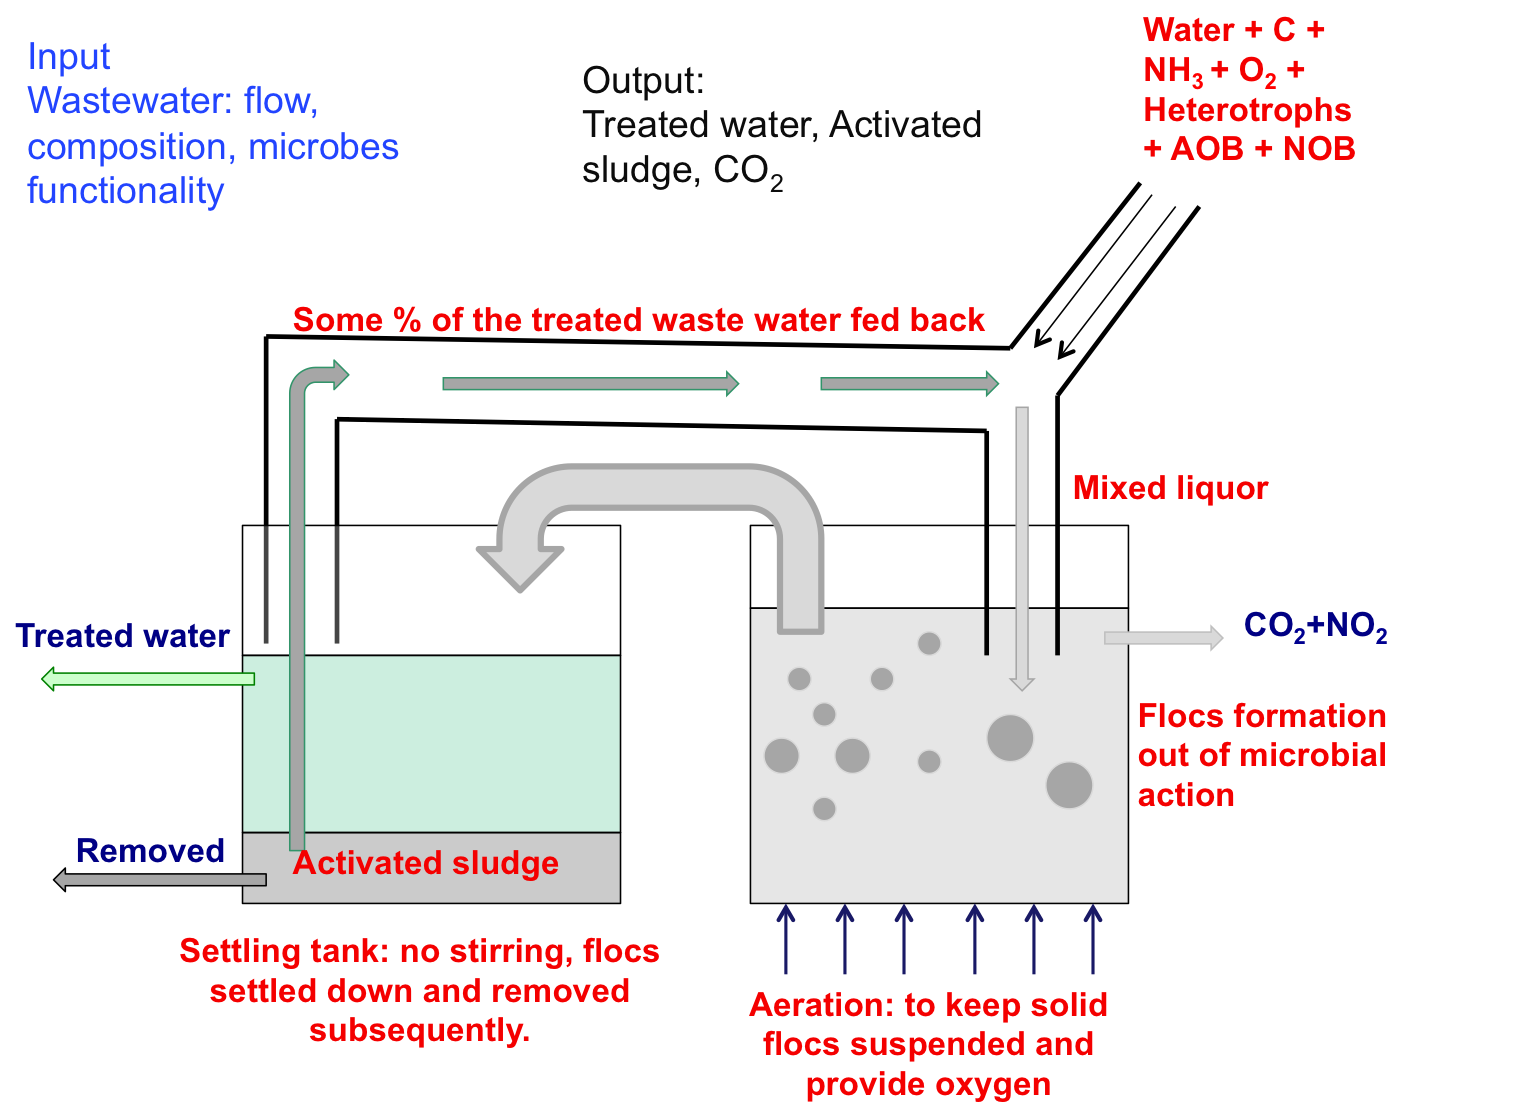
\includegraphics[width=0.75\columnwidth]{Figs/ASP.png}
\caption{Activated sludge process description for a waste water treatment plant (WWTP)}
\label{fig:ASP}       % Give a unique label
\end{center}
\end{figure} 


\subsection{Floc formation}
A floc is described as an aggregate of microbes bonded together by adhesive material (EPS) secreted by them. These clusters formations, often called as activated sludge, play a key role in the functioning of any waste water treatment plant (WWTP). Efficiency or the energy requirement of either of the primary and secondary tanks in an activated sludge process, depends upon the floc size, settlement or motility. Furthermore, the floc formation is governed by the microbial components adherence and cluster breakages.

\subsubsection{Biological process}
\subsubsection{Physical process}


\section{Individual based modelling (IBm)}
Pilot scale plants and laboratory scale experiments of WWTP are expensive, cumbersome, non-invasive and often can not provide information at the micro-scale, which is required for operational optimization of WWTP. Modelling of WWTP is challenging due to wide separation of temporal and spatial scales at which biological and physical processes key roles. Henceforth, a multi-scale modelling strategy is required to relate the microscopic microbial actions (often less than a micrometer size) to the macroscopic bulk WWTP operation (meter size scale). Identification of different length scales typical to a WWTP is presented can be shown in the figure \ref{fig:lscale}.  

\begin{figure}[!htb]
\begin{center}
  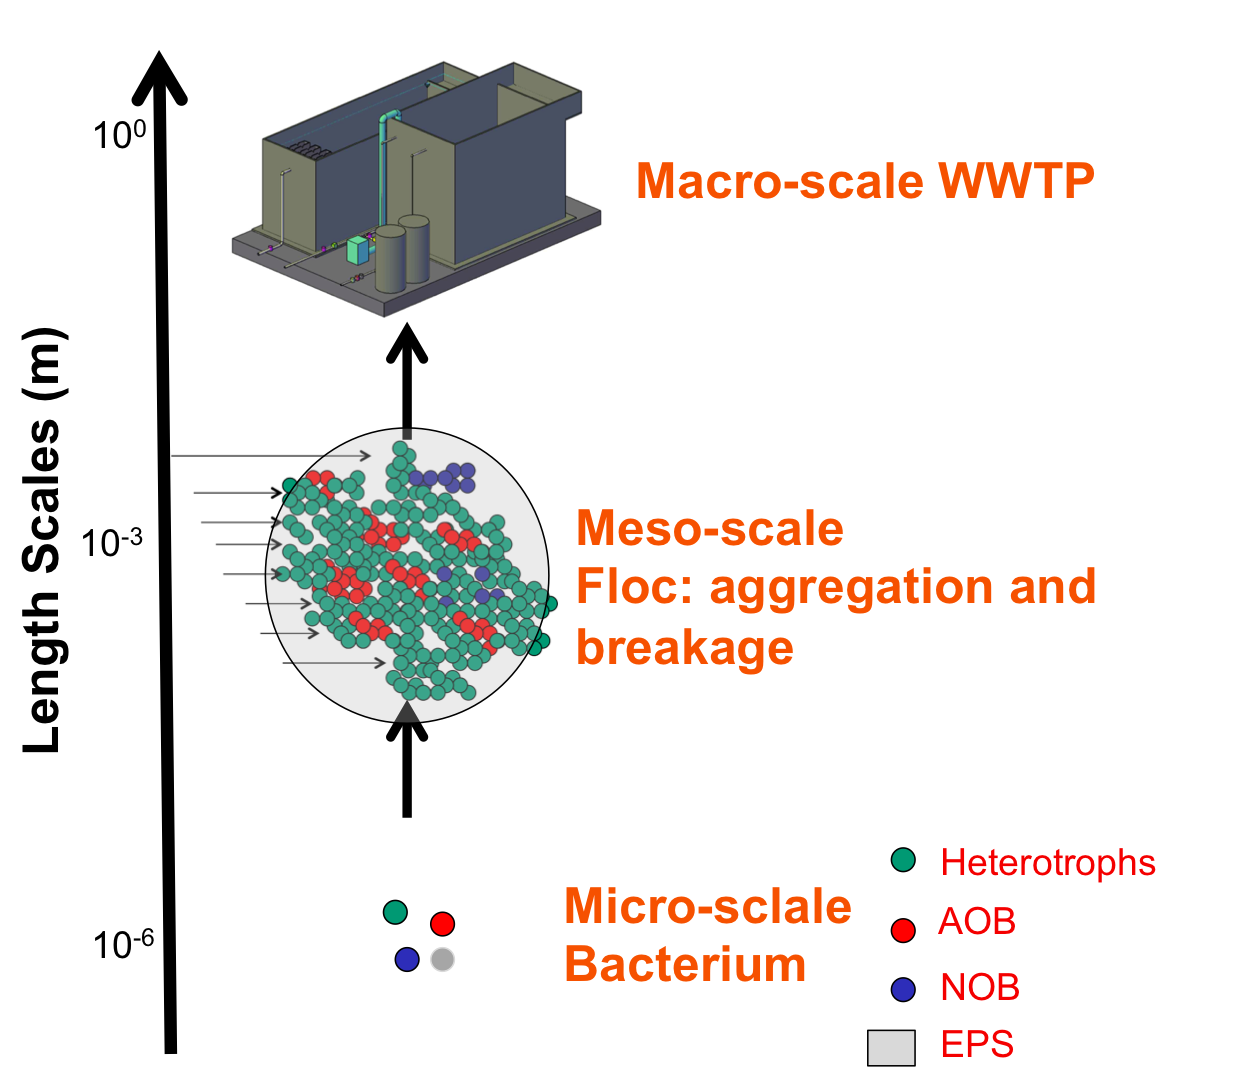
\includegraphics[width=0.5\columnwidth]{Figs/lengthscales.png}
\caption{Schematic of typical length scales for multi-scale modelling of a activated sludge process based Waste water treatment plant (WWTP)}
\label{fig:lscale}       % Give a unique label
\end{center}
\end{figure}  
 
\subsection{Introduction}
Discrete unit models such as the cellular automaton (Picioreanu et al., 1998a) or the individual-based models (Kreft et al., 1998), have been first developed and are now becoming widely applied to study effects of spatially multidimensional gradients in biofilms. Models which use individuals as a basic unit have occasionally been used in ecology since 1970s, but only since the visionary review of Huston et al. (1988) has individual-base modelling been an explicitly delineated approach of ecological modelling. Individual-based modelling refers in the following to simulation models that treat individuals as unique and discrete entities which have at least one property in addition to age that changes during the life cycle, e.g. weight, rank in a social hierarchy, etc. For biofilm modelling, Kreft et al. (1998, 2001) initially proposed the Individual-based Modelling (IbM) as a proper tool compared with existing Cellular Automaton (CA) method used for biofilm modelling. In CA models, the biofilm is represented by collection of bricks, in which each brick is represented by a Cartesian grid (Picioreanu et al., 1998a, 1998b,2000a; Knutson et al., 2005; Tang and Valocchi, 2013, Radu et al. 2010). In IbM, bacterial cells are represented as hard spheres, with each cell having, besides a variable volume and mass, a set of variable growth parameters, position, velocity, genotype etc. The IbM model consists of two parts: one deals with the growth and behaviour of individual bacteria as autonomous agents (i.e., biological processes); the other deals with the substrate and product diffusion and reaction and fluid flow (i.e., physical processes). Each cell grows by consuming the substrate and divides when a certain volume or mass is reached. The pressure build-up due to the growth of biomass is released by maintenance of a minimum distance between the neighbouring cells. In the traditional IbM approach, for each cell, the vector sum of all positive overlap radii with the neighbouring cells, which is called the shoving vector, is calculated and then the position of the cell is shifted in the direction opposite to this vector 3 sum. The substrate concentration is governed by a convection-diffusion-reaction equation and this transport equation is solved in a fixed Cartesian grid. Figure 1 shows the typical computation domain associated with IbM of biofilms. Basically it has three sub-domains each for biofilm, mass transfer boundary layer, and bulk fluid. Numerical simulations in 2D showed that the IbM produced a more confluent and rounded biofilm structures than the CA based models, due to its deterministic and directionally unconstrained spreading of the biomass (Wang and Zhang, 2010).


\subsection{Model description}

\subsection{Purpose of the model}

The model treats each microbes as individual entities interacting with each other and the surrounding environmental conditions. Various sub-models are employed for describing biology and physics at different length and temporal scales. 
The multi-physics/biological model developed can be used to investigate following key questions at different scales:

\begin{itemize}
\item Linking the microscopic (bacterium) to the mesoscopic (floc) to the macroscopic bulk operational parameters. 
\item Floc formation mechanism: How the microscopic phenomenon such as microbial growth kinetics, division, death, nutrient availability lead to microbial floc formation or breakage?
\item Effects of floc morphology and motility on the overall plant efficiency? 
\item How the hydrodynamics of the system can influence energy requirements of the WWTP?
\item Effect of the nutrient availability spatially and temporally?
\end{itemize}

\subsection{Model variables and principles}

The solver treats the microbes as spherical particles with EPS shells bounded on them. Fluid is treated as a continuum.
Nutrients are treated as concentrations in dissolved and convected through the flow fields. Given by their representations each components are solved accordingly. 

\begin{itemize}
\item Microbes: solved in a Lagragian framework. Each microbes is represented as a finite size sphere and has certain functionality. They are tracked throughout the simulations. The interactions between the microbes and with their ambient environment are complex and are described through different biological and physical sub-models described later. Following functional groups are considered: Heterotrophs (HET), Ammonia oxidizing bacteria (AOB), Nitrogen oxidizing bacteria (NOB), EPS particles and dead inert particles. 

\item Fluid: Fluid or the water phase is treated as a continuum media with microbes mostly suspended (neutrally buoyant). The fluid motion is solved in an Eulerian grid and takes into the account of the microbial suspension. Fluid and particle motion are tightly coupled by the hydrodynamics solver. 

\item Nutrients: The nutrients are treated as concentrations of the food supply in the water phase. The fluid solver supplies these nutrients to the microbes and hence contributes to their metabolism. Following nutrients relevant to the waste water treatment plant are taken into the account: Carbon substrates ($S_s$), Oxygen supply ($O_2$), Nitrates ($NO_{2}$), Nitrites ($NO_{3}$) and Ammonia ($NH_{4}$).
\end{itemize}

\subsection{IBm submodels}
Various cell level processes constitutes microbial working at cell level. Each of these processes can be termed as components of IBm model presented here. Modelling and fundamentals of each of these processes are presented here:

\subsubsection{Cell Growth}\label{growthmol}
Commonly found microbes in a WWTP can be grouped into functional group: Heterotrophs (HET), Ammonia oxidizing bacteria (AOB) and Nitrogen oxidizing bacteria (BOB). Each of the functional groups consume different nutrients and compete with each other for survival. Present tool allows a functional group and its function to be defined accordingly. Following equations give the reactions and their description is presented in a matrix form (\ref{fig:gdrates}):

\begin{equation}
\label{eq:GM}
\frac{dm_{i}}{dt} = Gm_{i}
\end{equation}

Each species has its own growth rate (G) and can be described according to the equation \ref{eq:GM12}. $\gamma_{HET} = 1$ and rest are zero, when solving for the HET equations. Same can be extended to AOB, NOB and EPS particles. $R_{j}$ (j=1-9) are given in the table \ref{fig:gdrates}.

\begin{equation}
\label{eq:GM12}
G = \gamma_{HET}\left ( R_1 + R_4 + R_5 \right )+\gamma_{AOB}\left ( R_2 \right ) + \gamma_{NOB}\left ( R_3\right ) -\gamma_{EPS}\left ( R_9\right )
\end{equation}

HET bound EPS growth rate is given by:
\begin{equation}
\label{eq:GMEPS}
G_{HET-EPS} = \frac{Y_{EPS}}{Y_{HET}} G m_{i}
\end{equation}

Reaction equations are primarily mass balance solved on the mesh discretization defined earlier. 

\begin{figure}[H]
\begin{center}
  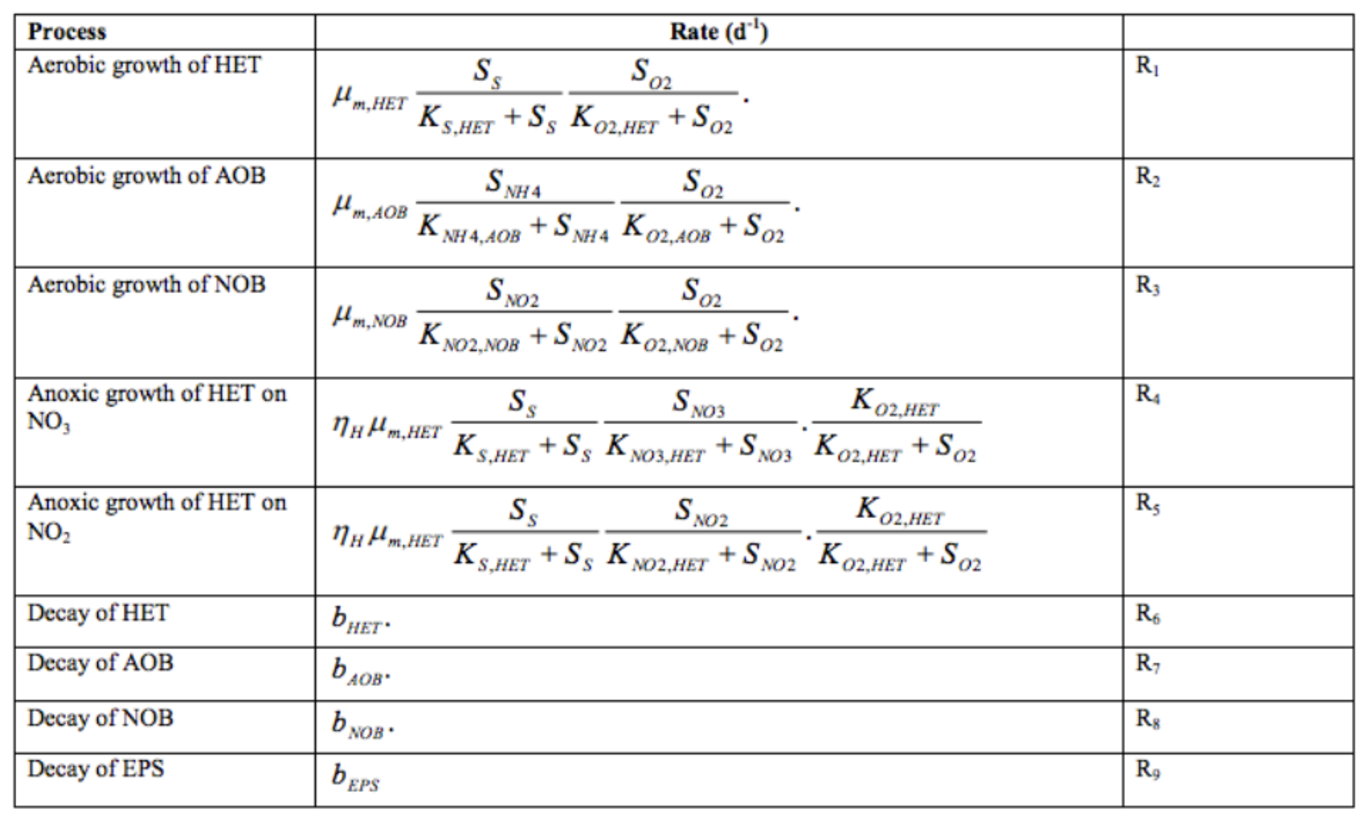
\includegraphics[width=0.9\columnwidth]{Figs/Tableforrates.pdf}
\caption{Growth and decay rates for AOB, NOB, HET and EPS particles.}
\label{fig:gdrates}       % Give a unique label
\end{center}
\end{figure}  


Each of the components of uptake or consumption is calculated separately and added together following superposition principle. The rate is defined according to Monod-kinetics where the kinetics factors are product together. Also, the rate of the growth/decay is proportional to the instantaneous mass of the substrate. The local nutrient availability for the growth of each cell is based upon the ambient conditions solved through the passive scalar transport of the nutrients. Fluid-biofilm coupling solver ensures that each cell is aware of its ambient nutrient conditions.Each of the cell has nutrient availability concentration attributes as: Soluble substrate (Ss), Oxygen ($O_2$), NO2, NO3, NH4. 

\subsubsection{Cell Division}\label{divisionmol}
Microbes can not grow forever (even with infinite food supply), division occurs due to sustenance of their sizes. Present model employs cell division rather empirically, by fixing up a maximum cell diameter, after which it divides. The model is implemented in following way: If the mass of a bacterial cell becomes greater than twice the mass of an inoculated individual bacterium, it divides into two daughter cells each. During the division process, the cell mass is split in a ratio randomly selected between 0.4-0.6. This generated two daughter cells from a parent cell. These daughter cells are oriented randomly around the centre of the parent cell. Figure \ref{fig:divcr} shows the division of daughter cells from the mother cell, randomly oriented around the centre of mother cell. This generation of newer particles occur at start of every time step and the forces equilibrated according to the overlaps, ensuring mechanical stability. The diameters of daughter cells are calculated using the cell mass and biomass density. Biomass density is constant for each species. 

\begin{figure}[H]
\begin{center}
  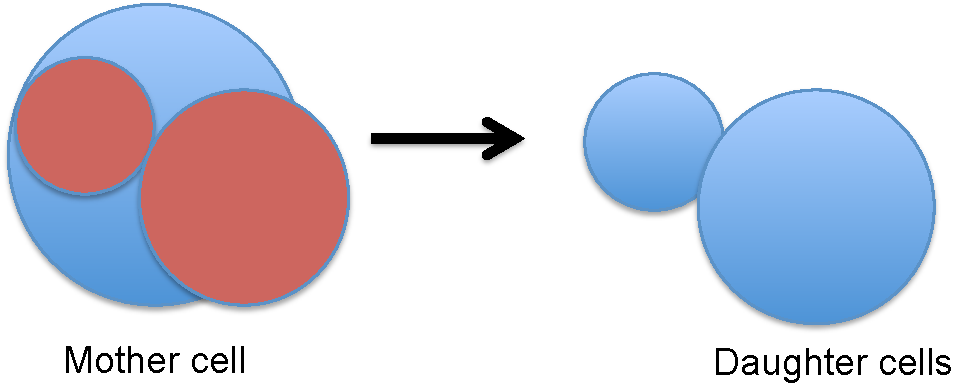
\includegraphics[width=0.6\columnwidth]{Figs/Divisioncrit.pdf}
\caption{Division of daughter cells from the mother cell, randomly oriented around the centre of mother cell}
\label{fig:divcr}       % Give a unique label
\end{center}
\end{figure}  


\subsubsection{Cell Death}\label{deathmol}
Microbial death is modelled as a random stochastic process. Every so often, a few microbes becomes biologically inactive i.e. they would not consume nutrient, grow or divide. These cells are treated as inactive particles by the solver and only participate in any physical/mechanical interactions with their neighbours. Depending on the total decay mass of HET, AOB, and NOB, the appropriate numbers of HET, AOB, and NOB cells are calculated and died. The mass of the dying cell shares between dead cell and carbon source. The mass of decaying EPS cells totally converts to carbon. Completely dissolved EPS particles are removed from the calculation. In the model this implemented by the total virtual dead mass of each species (HET or AOB or NOB) and is calculated from equations as below:

\begin{equation}
\label{eq:DR}
D = \gamma_{HET}R_{6} + \gamma_{AOB}R_{7} + \gamma_{NOB}R_{8}
\end{equation}

\begin{equation}
\label{eq:DR1}
M_{virtual} = \sum Dm
\end{equation}

where, D is the decay rate. At each time step (dt), number of cells equivalent to $M_{virtual}$ is set as dead (i.e. ID is changed to 5). These particles are randomly selected. When a cell is died, Y fraction of its mass remains in the dead cell and the other fraction (1-Y) is spontaneously converted to carbon substrate ($S_s$) and distributed to the Cartesian grid cell centre in which the particle resides. 

\subsubsection{EPS production and excretion}\label{EPSmol}
Microbes secrete extracellular polymeric substances (EPS) every so often as a waste product of their metabolic activities. EPS is secreted into their neighbouring environment and have known to lend structural integrity to the biofilms. Previous solvers have represented EPS in continuum and discrete manner. The solver works on the common knowledge that HETs excrete EPS, while AOB and NOB microbes do not. The present solver follows the iDynnomics approach of EPS treatment. Initially, EPS is accumulated as a extra shell beyond the HET particle (figure \ref{fig:EPScr}). It should be noted that the EPS density is much lower than the HET density. When the relative thickness of the EPS shell bound to HET particle exceeds a certain threshold value, almost half (random ratio between 0.4-0.6) of the EPS mass excretes as a separate EPS particle and positions next to the HET cell.

\begin{figure}[H]
\begin{center}
  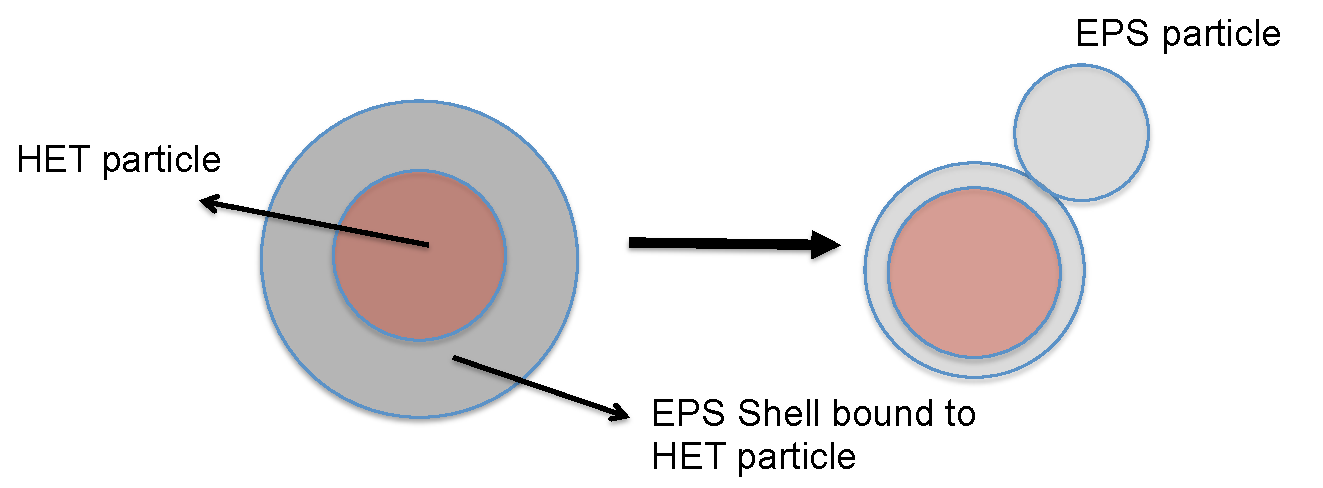
\includegraphics[width=0.6\columnwidth]{Figs/EPScrit.pdf}
\caption{EPS bound to the the HET particle, extracted to an EPS particle according to the ratio between the EPS shell and the HET particle radius.}
\label{fig:EPScr}       % Give a unique label
\end{center}
\end{figure}  

\subsubsection{EPS-Adhesion forces}\label{adhmol}
The excreted EPS mass from the HET particles can be employed as a parameter of adhesion force models between the particles. The EPS link between the particles are treated as much more stiffer springs, but only employing the attractive forces. Total effective EPS mass is calculated between the microbes ($Meps_{eff}$) and a spring stiffness is defined per unit mass ($k_{eps}$). Effective overlap between the EPS links are calculated and the forces calculated according to the effective spring stiffness ($Meps_{eff}$*$k_{eps}$) multiplied by the overlap. This approach was first applied by Head et al. to reproduce a mechanically stable biofilm. 


\subsection{Stochastic processes: Scope of improvement}
Different processes are modelled by the sub-models as stochastic processes. This adds variability and randomness to the biological process, typically evident in the nature. Following processes are random:

\begin{itemize}
\item Initialization of the system by placing the microbes with random physical and biological attributes are placed at random locations within the domain. This introduces the randomness of the initial configuration. 

\item Cell division criterion is based on a critical random maximum ratio, which can be selected by the user. Solver further divides the daughter cell masses randomly in a ratio between 0.4-0.6 placing daughter cells in a random orientation. 

\item During the death sub-model, microbes equivalent to the dead-mass are randomly chosen by the solver. 

\item EPS excretion occurs after the shell bound EPS exceeds a randomly selected value by the user. This excreted EPS is oriented and placed randomly around the mother cell. 

\end{itemize}

As recommended by the iDynomics solver, these processes can be tackled from a microscopic point of view with fundamental chemical and biological processes driving these mechanisms.   

%\subsection{Modelling bio-film dynamics and response to the fluid flow}
%\begin{itemize}
%\item Physical processes in a activated sludge process. 
%\item Typical forces acting on a bio-particle. 
%\item how to model them. 
%\item Hydrodynamics of the system. 
%\end{itemize}
%
\section{LAMMPS}
\subsection{Introduction to LAMMPS}
LAMMPS is a classical molecular dynamics code developed at Sandia labs and primarily built to solve the particle physics including wide range of inter-particle interactions and potentials. The code treats each particle as an individual discrete unit, much similar to the popular IB approach. Sandia Labs distributes LAMMPS under the terms of the GNU Public License (http://lammps.sandia.gov/). The current version of the code is written in C++ with an open architecture and provides an opportunity to couple with other open-source codes. LAMMPS can run efficiently in both serial and parallel versions depending upon the computational facilities available to the users.  The LAMMPS code is designed to modify and extend it with newer capabilities as desired by the user. While only 25 percent of the 140K line code in LAMMPS forms the core of the solver, rest of the code is contributed by a large user database across the globe in order to extend its capabilities. An overview can of current LAMMPS capabilities can be found at \href{http://lammps.sandia.gov/features.html}{LAMMPS-feature}.

\subsection{LAMMPS working methodology}
LAMMPS solves the motion of every single particle by simply integrating Newton's equations of motion in response to sum of the forces (short or long range based on their interaction with neighbours). At a particular time instance, motion of each particle is collectively solved when subjected to initial or boundary conditions. In order to maintain computational tractability while calculating the interaction forces, LAMMPS maintains a neighbourhood list for each particle which gets updated every so often. These lists are optimized so that local densities and particle overlaps never becomes non-physical. For parallel simulations, LAMMPS spatially partition the domain into smaller sub-domains assigned to each processors. Interprocessor communications are maintained by storing ghost atom interactions with the sub-domain boundaries. LAMMPS development can be helped by two user manuals: User manual and developer manual. The following links will be helpful for the users to get started on LAMMPS:

\begin{enumerate}
\item User manual: \url{http://lammps.sandia.gov/doc/Manual.pdf}
\item Developers guide: \url{http://lammps.sandia.gov/doc/Developer.pdf}
\item Tutorials: \url{http://lammps.sandia.gov/tutorials.html}
\item Commands: \url{http://lammps.sandia.gov/doc/Section_commands.html}
\item Features: \url{http://lammps.sandia.gov/features.html}

\end{enumerate}

%A further overview on LAMMPS can be taken from: $http://lammps.sandia.gov/tutorials/italy14/italy_overview_Mar14.pdf$
In the present study, LAMMPS-Feb14 version is developed and newer IB features and capabilities added, this version will be now on referred as LAMMPS-NCL. 

\subsection{Operating systems}
In general, LAMMPS can be run on Windows, Linux, Mac OS using pre-built executables. LAMMPS-NCL can be compiled with almost any linux or Mac OS (instructions in the user manual). It is emphasized that present NCL version has been rigorously tested on Ubuntun-14.10 and Fedora-22. In near future, prebuilt executables,binaries or RPMS will be provided to be used on any OS.

\subsection{Pre-compilation instructions}

Before compiling LAMMPS, please make sure you are installed with these packages depending upon the operating system used:

\begin{itemize}
\item fftw (http://www.fftw.org/doc/Installation-on-Unix.html)
\item openmpi (http://www.open-mpi.org/)
\item libjpegm (http://libjpeg-turbo.virtualgl.org/)
\item gcc/g++ (https://help.ubuntu.com/community/InstallingCompilers)
\end{itemize} 

\section{LAMMPS-NCL and getting started}

For the pre-existing LAMMPS commands, features and documentation, please refer to the LAMMPS user manual, listed above. The manual covers extensive instructions on compiling LAMMPS and how to get started. LAMMPS-NCL is compiled the same way as you would compile LAMMPS and there is no change in those instructions. The newer capabilities and commands will be highlighted and emphasized in the next sections and the sample input script.  


\subsection{Downloading LAMMPS-NCL}
In general, different versions of LAMMPS can be downloaded from the \href{http://lammps.sandia.gov/download.html}{download section} of the LAMMPS website. For the present study, LAMMPS version Feb 2014 was developed and enhanced with biological IB model capabilities. It is advised to use the version developed at NCL. It can be downloaded using following set of instructions from the NUFEB Github repository.


\subsection{LAMMPS extension}
In the present study, capabilities of LAMMPS have been extended to include cell level biological processes such as cell growth, division, maintenance, death etc. These extended capabilities involve addition of newer particles at each time-steps e.g. during a cell division: a single parent cell divide into two daughter cells. A summary of list of newer capabilities added to the LAMMPS and its implementation is presented here:


\subsection{Atom type}
Classical LAMMPS provide different atom types that could be used by user. These are specified in the input script by the command: \href{http://lammps.sandia.gov/doc/atom_style.html}{$atom-style$}. \href{http://lammps.sandia.gov/doc/atom_style.html}{$atom-style$} command must be used before a simulation is setup via a \href{http://lammps.sandia.gov/doc/read_data.html}{read-data}, \href{http://lammps.sandia.gov/doc/read_restart.html}{read-restart} or \href{http://lammps.sandia.gov/doc/create_box.html}{create-box} command. A newer $atom-style$ is added (named "bio") to increase the number of attributes such as nutrients available to each microbe type. The new $atom-style$ is inherited from already existing $atom-style$ sphere. Though LAMMPS provides another route for adding newer attributes through \href{http://lammps.sandia.gov/doc/fix_property_atom.html}{fix property/atom}. However, since the newer attributes would be used to couple with the fluid solver, they should be more tightly linked to the atom style. 

The new atom type "Bio" have following attributes in conjunction to the sphere type: ID, type, radius, outerradius, mass, outermass,x,y,z, $S_s$, $O_2$, $NO_3$, $NO_2$, $NH_4$. As a general rules following types are assigned to the functional groups. 

\begin{itemize}
\item 1-HET 
\item 2-AOB
\item 3-NOB
\item 4-EPS
\item 5-Inert
\end{itemize} 

Each microbe has unique moniker ID but share its type according to the functional group. Physical parameters such as initial radius, outer radius, density and outer density can be mentioned. Radius and density are the radius and density of the microbe. Outer radius and densities are the initial EPS-shell bound radius and densities. Density is constant throughout the simulation and time invariant. However radius and mass (calculated from density and radius) can change. EPS is only bound to the HET particles (type 1), hence outer radius should be specified as radius for other particle types initially. LAMMPS will give an error message if this is not followed. For LAMMPS book-keeping, inner radius is always same as outer-radius for other types than 1 throughout the simulation. Initial configuration can be either generated randomly through LAMMPS or by the user. Caution must be taken to avoid overlaps when defined by the user. A typical user input script is included in the folder (IC5nut.in). 

Different sub-models are coded within LAMMPS in a modular way. Each of these models, implementations and command lines are explained in the following sub-sections.


\section{Input script generated for the NUFEB-Bio simulations}
In order to execute LAMMPS commands, an input script is usually prepared with certain sub-commands and parameters list. 
Figure \ref{fig:inputscript} gives the input script for the NUFEB project. This script can be generated by GUI and will be explained later. New additions to the LAMMPS commands are pointed in the boxes as shown in the figure. 

\begin{figure}[H]
\begin{center}
  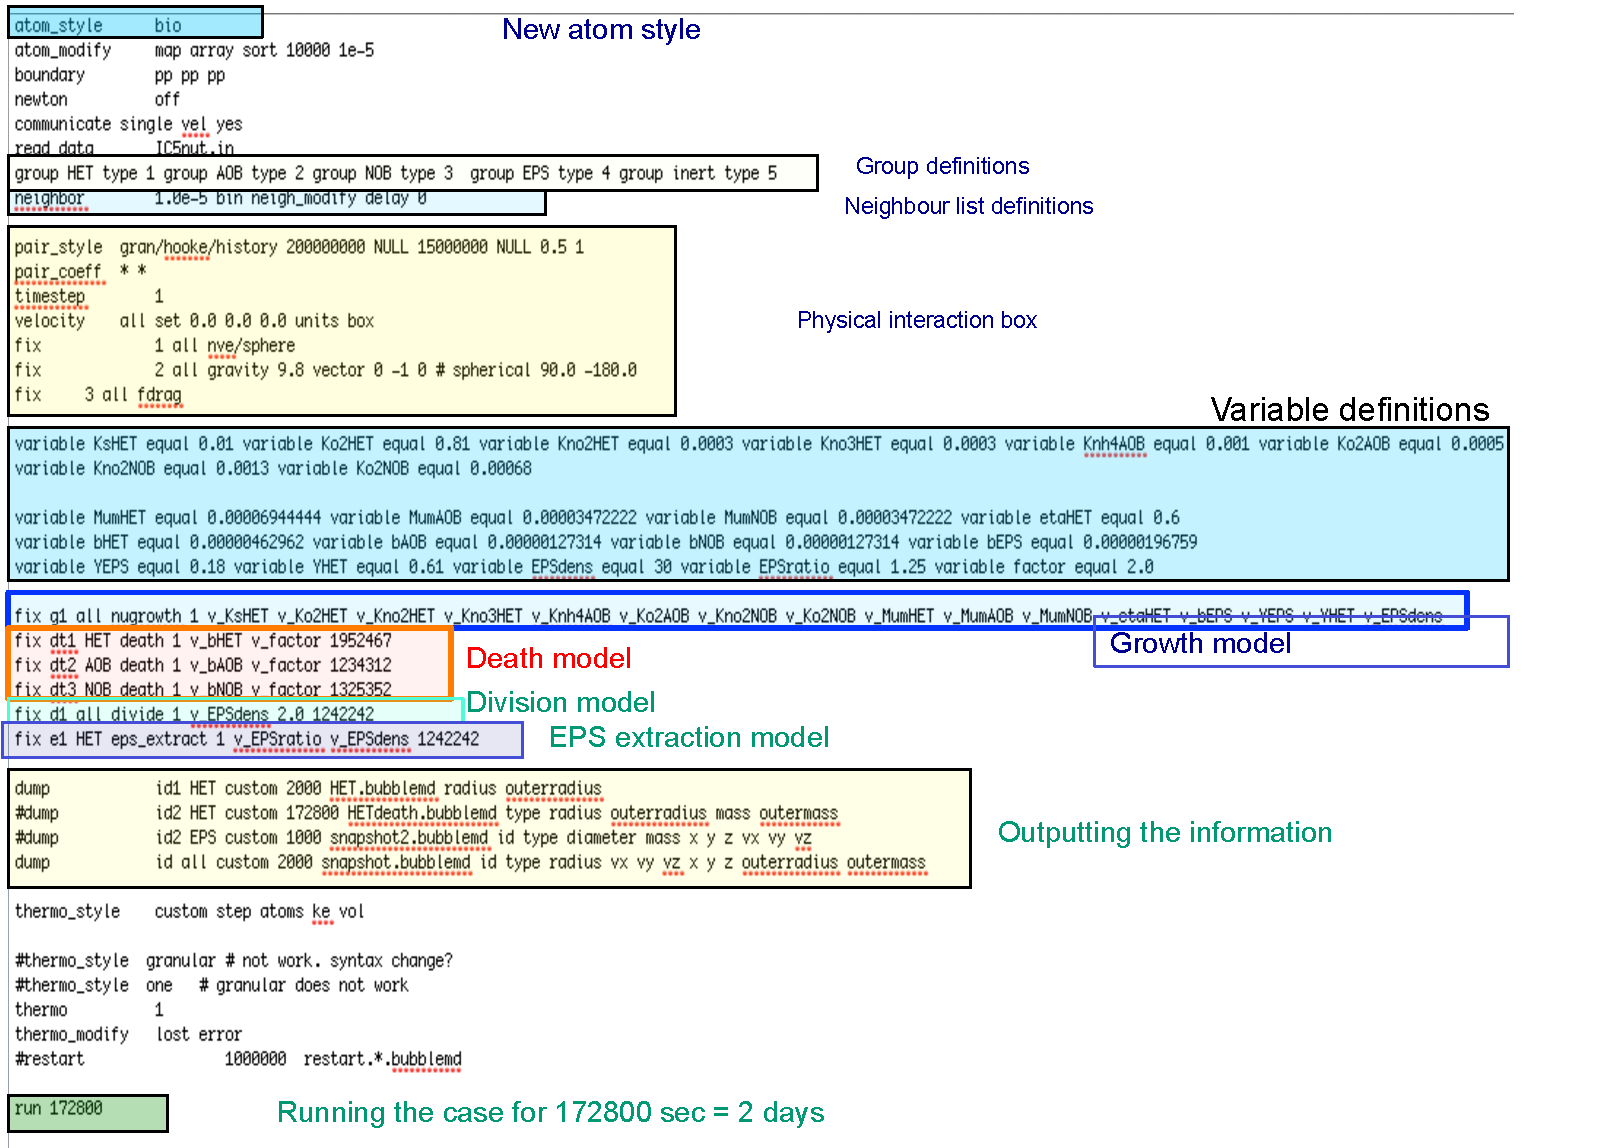
\includegraphics[width=0.9\columnwidth]{Figs/Inputscript.pdf}
\caption{Input script for NUFEB simulation of biofilm dynamics.}
\label{fig:inputscript}       % Give a unique label
\end{center}
\end{figure}  


\subsection{Cell growth}
Cell growth model described in the section \ref{growthmol} is implemented as a fix type "growth" in the LAMMPS, the source code can be found in the src folder of the LAMMPS directory. In the present implementation, GUI will help to generate LAMMPS command line for the fix growth and user just have to make sure to put in correct parameters. GUI is described later. Figure \ref{fig:growth} gives the LAMMPS command line for the growth model.

\begin{figure}[H]
\begin{center}
  
\includegraphics[width=0.98\columnwidth]{Figs/growthfix.pdf}
\caption{Command line for the growth fix in LAMMPS}
\label{fig:growth}       % Give a unique label
\end{center}
\end{figure}
 
In total, 20 parameters are given for the growth fix command. Specifically, "fix g1 all nugrowth 1" means invoke a fix nugrowth instance named g1 and apply it at everytimestep (1 = frequency of call) to "all" the particle types in the assembly. The second parameter "all" indicates that all the microbes can grow. Any other microbial type could also be mentioned, which would indicate that growth only occurs only for that specific type. All of the parameters has to be in SI units. A table of the typical parameters can be seen at the end of the documentation. The parameter description:

\begin{itemize}
\item fixID: unique ID of the fix (not used in the script before)
\item group: Functional groups on which fix will be invoked, it can take: HET, AOB, NOB, all.
\item fix-name: nugrowth (fix name). It can not take another value.
\item freq: frequency at which the fix is invoked (typically at every timestep). Values has to be integers.
\item KsHET Ko2HET Kno2HET Kno3HET Knh4AOB Ko2AOB Kno2NOB Ko2NOB: Affinity of all the functional groups to the substrate.
\item MumHET MumAOB MumNOB: Monod kinetic parameters for the HET, AOB and NOB.
\item etaHET: Reduction factor in anoxic conditions for HET.
\item bEPS: Decay rate of EPS.
\item YEPS, YHET: Yield coefficient for EPS and HET particles.
\item EPS-density: Density of the EPS, required for the divisions of HET particles. Values can be floating type number.
\end{itemize}


\subsection{Cell Division}
Cell division model described in the section \ref{divisionmol} is implemented as a fix type "division" in the LAMMPS, the source code can be found in the src folder of the LAMMPS directory. The command line is given in the figure \ref{fig:division}:

\begin{figure}[H]
\begin{center}
  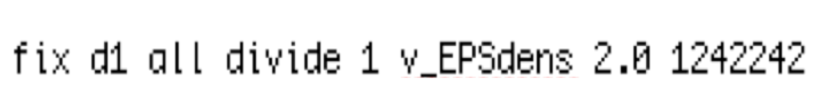
\includegraphics[width=0.6\columnwidth]{Figs/divisionfix.pdf}
\caption{Command line for the division fix in LAMMPS}
\label{fig:division}       % Give a unique label
\end{center}
\end{figure}

The command line follows the template: "fix fixID group fix-name freq EPS-density Ratio seed". The parameter description:
\begin{itemize}
\item fixID: unique ID of the fix (not used in the script before)
\item group: Functional groups on which fix will be invoked, it can take: HET, AOB, NOB, all.
\item fix-name: divide (fix name). It can not take another value.
\item freq: frequency at which the fix is invoked (typically at every timestep). Values has to be integers.
\item EPS-density: Density of the EPS, required for the divisions of HET particles. Values can be floating type number.
\item Ratio: User defined diameter ratio at which the division takes place. The ratio is calculated as the instantaneous diameter divided by the average diameter of the microbes. The average diameter is initially defined and hard coded. The values have been indicated in the earlier sections. Values typically floating type number greater than 1.0.
\item Seed: Seed for the orientation and introduce the randomness, very large integer values. Same seed will result in the same orientation for every simulation run. 
\end{itemize}

\subsection{Cell Death}
Cell death model described in the section \ref{deathmol} is implemented as a fix type "death" in the LAMMPS, the source code can be found in the src folder of the LAMMPS directory. Figure \ref{fig:death} gives the specific command lines.

\begin{figure}[H]
\begin{center}
  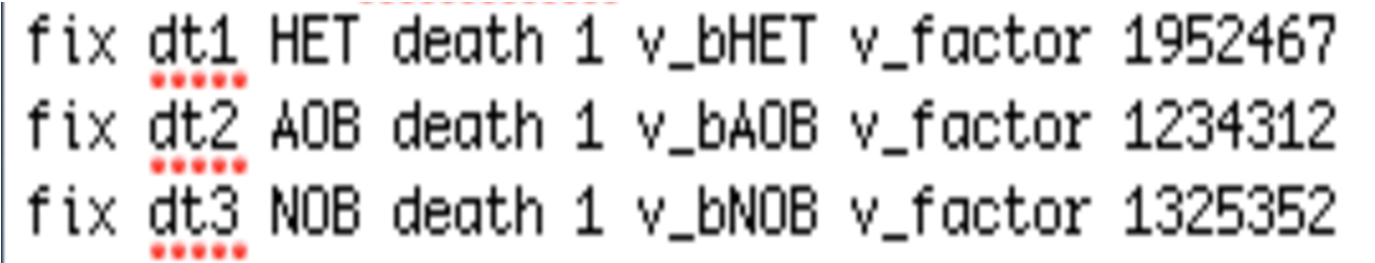
\includegraphics[width=0.6\columnwidth]{Figs/deathfix.pdf}
\caption{Command line for the death fix in LAMMPS}
\label{fig:death}       % Give a unique label
\end{center}
\end{figure}

The command line follows the template: "fix fix-ID group fix-name freq decay-rate ratio seed". The parameter description:
\begin{itemize}
\item fixID: unique ID of the fix (not used in the script before)
\item group: Functional groups on which fix will be invoked, it can take: HET, AOB, NOB, all.
\item fix-name: death (fix name). It can not take another value.
\item freq: frequency at which the fix is invoked (typically at every timestep). Values has to be integers.
\item decay-rate: Rate of decay, according to the type of microbe.
\item Ratio: Death ratio, described earlier in the model, typically floating number greater than 1.0.
\item Seed: Seed for randomly choosing particles to kill. 
\end{itemize}

\subsection{EPS extract}
EPS extraction model described in the section \ref{EPSmol} implemented as a fix type "EPS extract" in the LAMMPS, the source code can be found in the src folder of the LAMMPS directory. Figure \ref{fig:EPS} gives the specific command lines.

\begin{figure}[H]
\begin{center}
  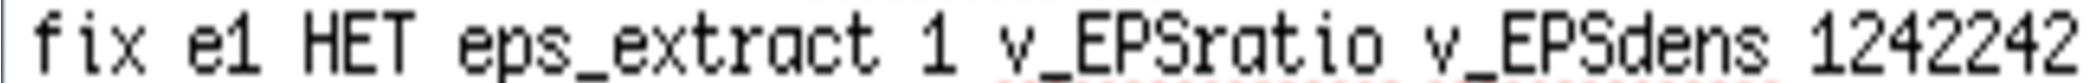
\includegraphics[width=0.6\columnwidth]{Figs/EPSfix.pdf}
\caption{Command line for the EPS extract fix in LAMMPS}
\label{fig:EPS}       % Give a unique label
\end{center}
\end{figure}

The command line follows the template: "fix fix-ID group epsextract freq EPSratio EPSdens seed". The parameter description:
\begin{itemize}
\item fixID: unique ID of the fix (not used in the script before)
\item group: Functional groups on which fix will be invoked, it can take: HET, AOB, NOB, all.
\item fix-name: death (fix name). It can not take another value.
\item freq: frequency at which the fix is invoked (typically at every timestep). Values has to be integers.
\item EPS ratio: Ratio between outer-radius and inner-radius of the microbe. Value is typically floating number greater than 1.0.
\item EPS-density: Density of the EPS, required for the divisions of HET particles. Values can be floating type number.
\item Seed: Seed for the orientation and introduce the randomness, very large integer values. Same seed will result in the same orientation for every simulation run.
\end{itemize}

\section{How to run a case}
Describe GUI.


%\section{References}

\label{References}
%\setlength{\bibsep}{3.0pt}
%\lhead{\emph{References}}  % Change the left side page header to "Bibliography"
%\rhead{\emph{References}}  % Change the left side page header to "Bibliography"
\small
%\begin{spacing}{0.9}
\bibliographystyle{Thesisnew}  % Use the "unsrtnat" BibTeX style for formatting the Bibliography
\bibliography{LAMMPS-Bio-Doc}  % The references (bibliography) information are stored in the file named "Bibliography.bib"
%\end{spacing}


\end{document}
